\documentclass{article}
\usepackage[T1]{fontenc}
\usepackage{lmodern}
\usepackage{graphicx}
\usepackage{amsmath,amssymb}
\usepackage[a4paper,margin=2cm]{geometry}
\usepackage[absolute,overlay]{textpos}
\setlength{\TPHorizModule}{1mm}
\setlength{\TPVertModule}{1mm}
\usepackage[indonesian]{babel}
\usepackage{hyperref}
\setlength{\emergencystretch}{2em}
% unit: Halaman 90

\begin{document}

% === Halaman 90 (llm) ===

\vspace{255.42mm}

python
def ProgramSteganografiAudio():
    print("-- Steganografi pada file audio WAV --")
    print("1: Penyisipan pesan")
    print("2: Ekstraksi pesan")

    pilih = input()
    if pilih == '1':
        print("Masukkan nama file audio WAV (beserta path-nya)")
        cover = input()
        print("Ketikkan pesan yang akan disisipkan ke dalam citra")
        pesan = input()
        print("Masukkan nama file audio WAV (stego audio) beserta path-nya")
        stego = input()
        print("Penyisipan pesan... (tunggu dengan sabar)")
        EmbeddingPesan(cover, pesan, stego)
    elif pilih == '2':
        print("Masukkan nama file audio stego beserta path-nya")
        stego = input()
        print("Ekstraksi pesan... (tunggu dengan sabar)")
        EkstraksiPesan(stego)
    else:
        print("Pilihan salah")

% deskripsi: Screenshot potongan kode program Python untuk steganografi audio
% bbox normalisasi: [0.0400, 0.0400, 0.9600, 0.9000]
\begin{textblock*}{193.20mm}(8.40mm,11.88mm)
\noindent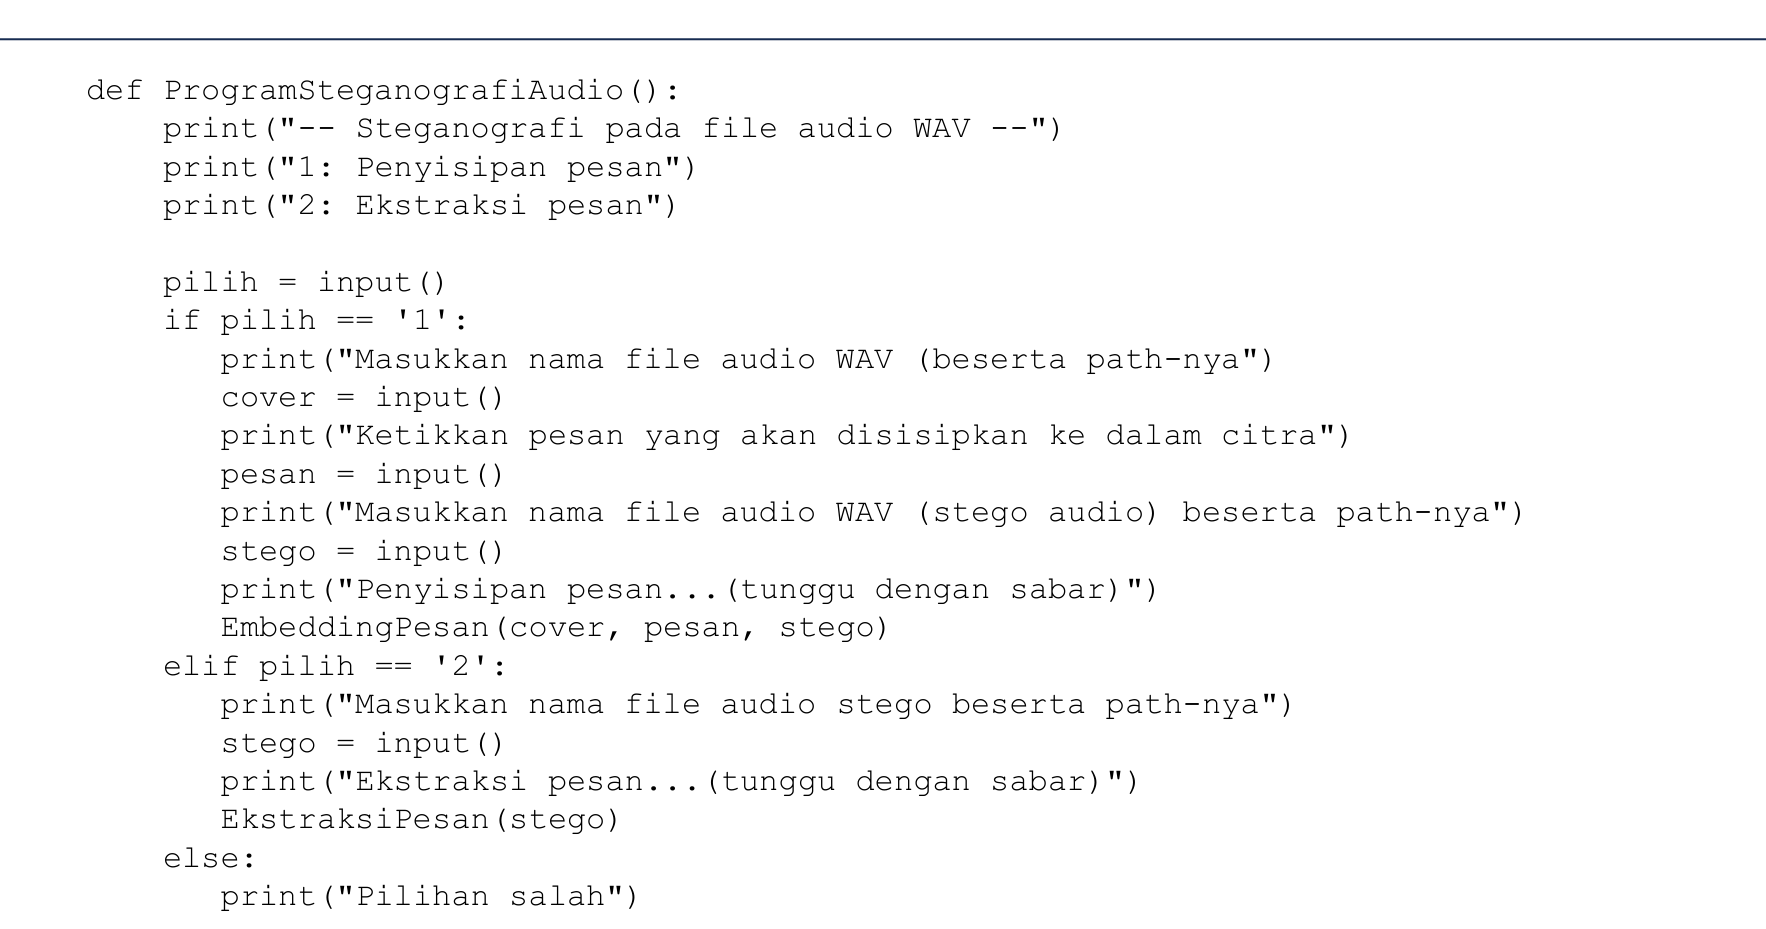
\includegraphics[width=193.20mm,height=255.42mm]{../../images/llm/page_090_img_01.png}%
\end{textblock*}

\end{document}
